\documentclass[]{article}
\usepackage[pdftex,paperwidth=436pt,paperheight=298pt,noheadfoot,left=0pt,top=0pt]{geometry}
\usepackage{graphicx}

\begin{document}
\noindent
%\scalebox{0.8819}[0.8966]{
\begin{picture}(434,297)
\put(-108,-428){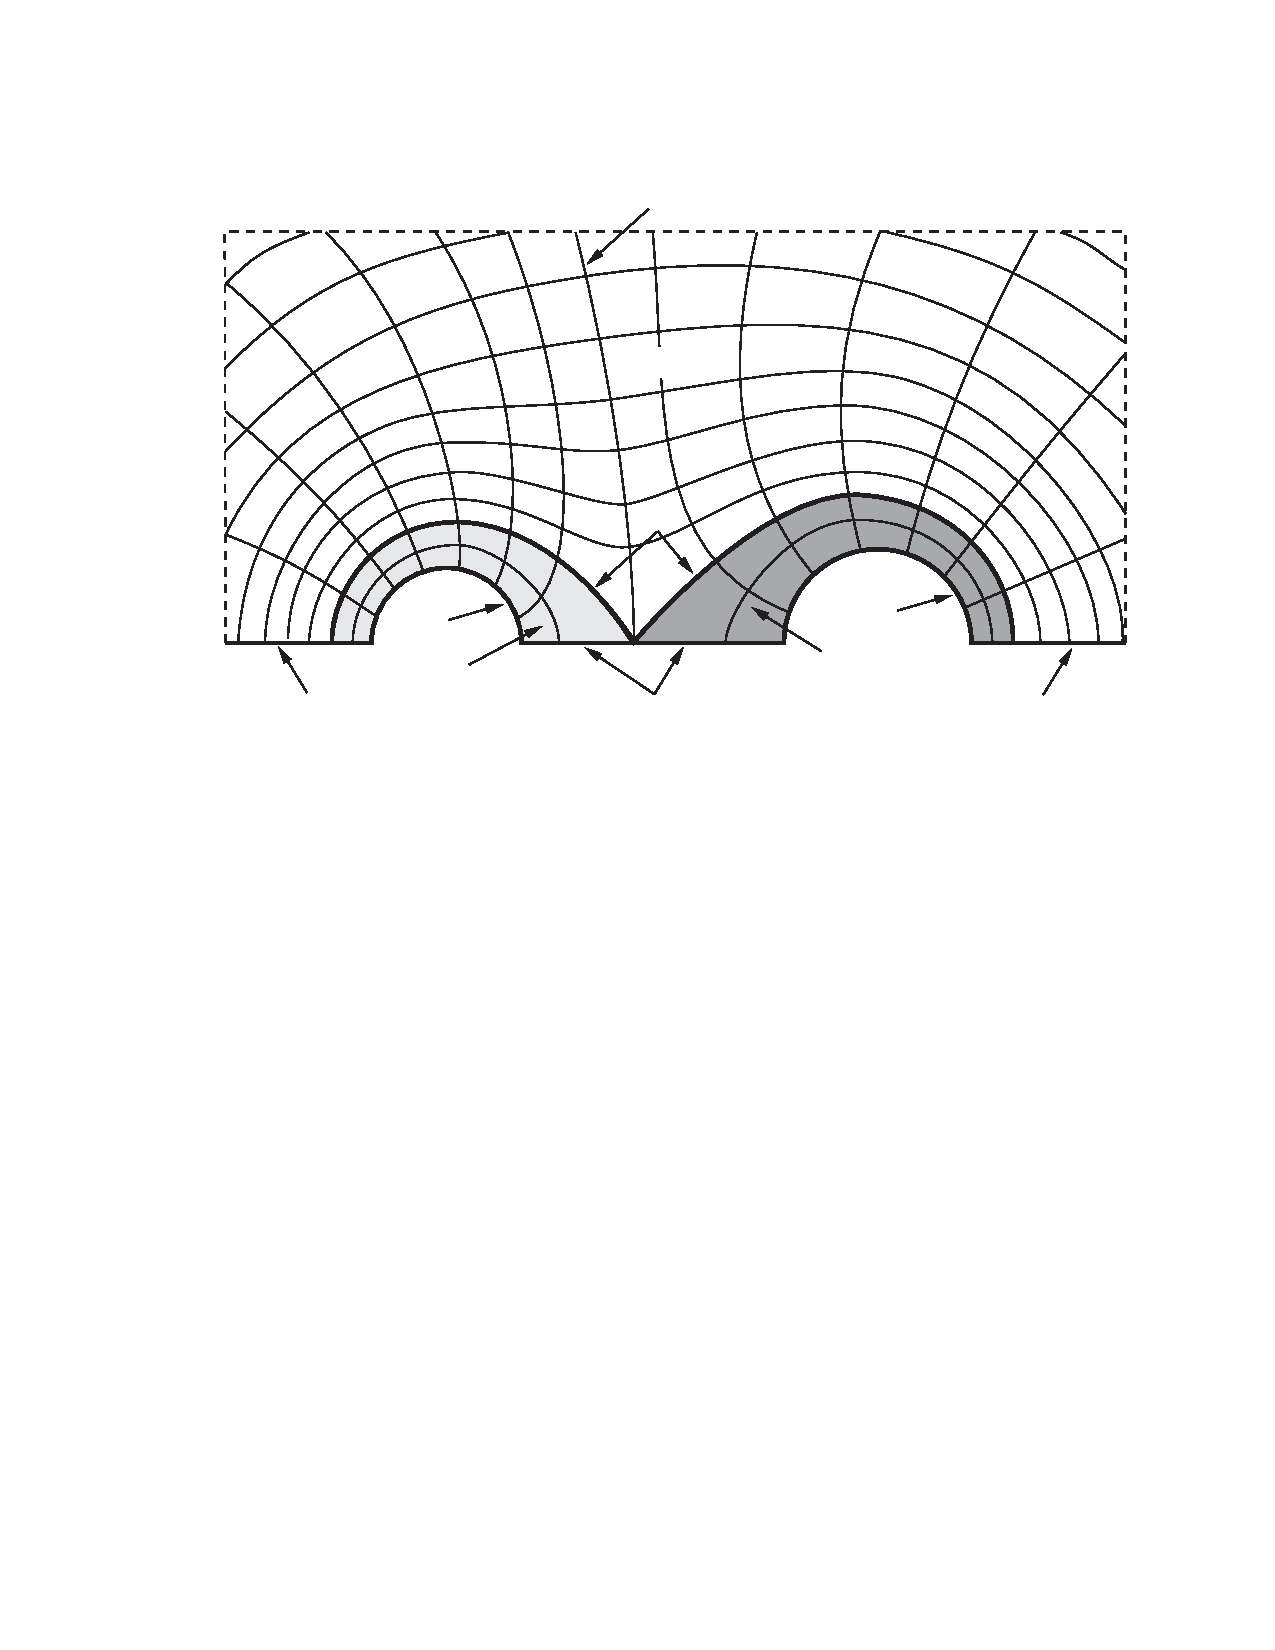
\includegraphics[width=8.5in]{PDFnotext/Figure10_1.pdf}}
\put(316,72){$\eta^+$}
\put(100,67){$\eta^-$}
\put(204,116){$\eta_s$}
\put(382,24){$\xi=0$}
\put(30,24){$\xi=\pi$}
\put(205,267){$\xi_s$}
\put(202,24){$\xi_s$ (double image)}
\put(280,42){Region 1}
\put(94,38){Region 2}
\put(193,189){Region 3}
\end{picture}
%}
\end{document}
